%!TEX root = ../rapport.tex
%!TEX encoding = UTF-8 Unicode

% Chapitres "Introduction"

% modifié par Francis Valois, Université Laval
% 31/01/2011 - version 1.0 - Création du document

\chapter{Modélisation de l'alimentation électronique}
\section{Fonctionnement d'un redresseur monophasé simple alternance}
Cette section a pour objectif de décortiquer le fonctionnement d'un redresseur monophasé simple composé d'une source de courant sinusoïdale parfaite, d'un interrupteur de type IGBT et d'une charge quelconque. Le montage analysé est présenté à la figure\ref{fig:RedresseurMonophaseSimpleAlternanceIGBT}. Pour les besoins de l'exemple, une charge $RL$ théorique sera utilisée. La résistance est dénotée par $R$ et l'inductance par $L$. De plus, on suppose que l'interrupteur IGBT entre en conduction lorsqu'un échelon de tension unitaire est appliqué à la grille de celui-ci, on le modélise comme un interrupteur idéal. Finalement, en supposant des modèles sans pertes, l'équation de circuit se résume à celle présentée à l'équation \ref{eq:RLSimple}. À noter que l'échelon unitaire est défini comme: $u(t<0) = 0, u(t\geq 0) = 1)$.

\begin{figure}[htb!]
	\begin{center}  
		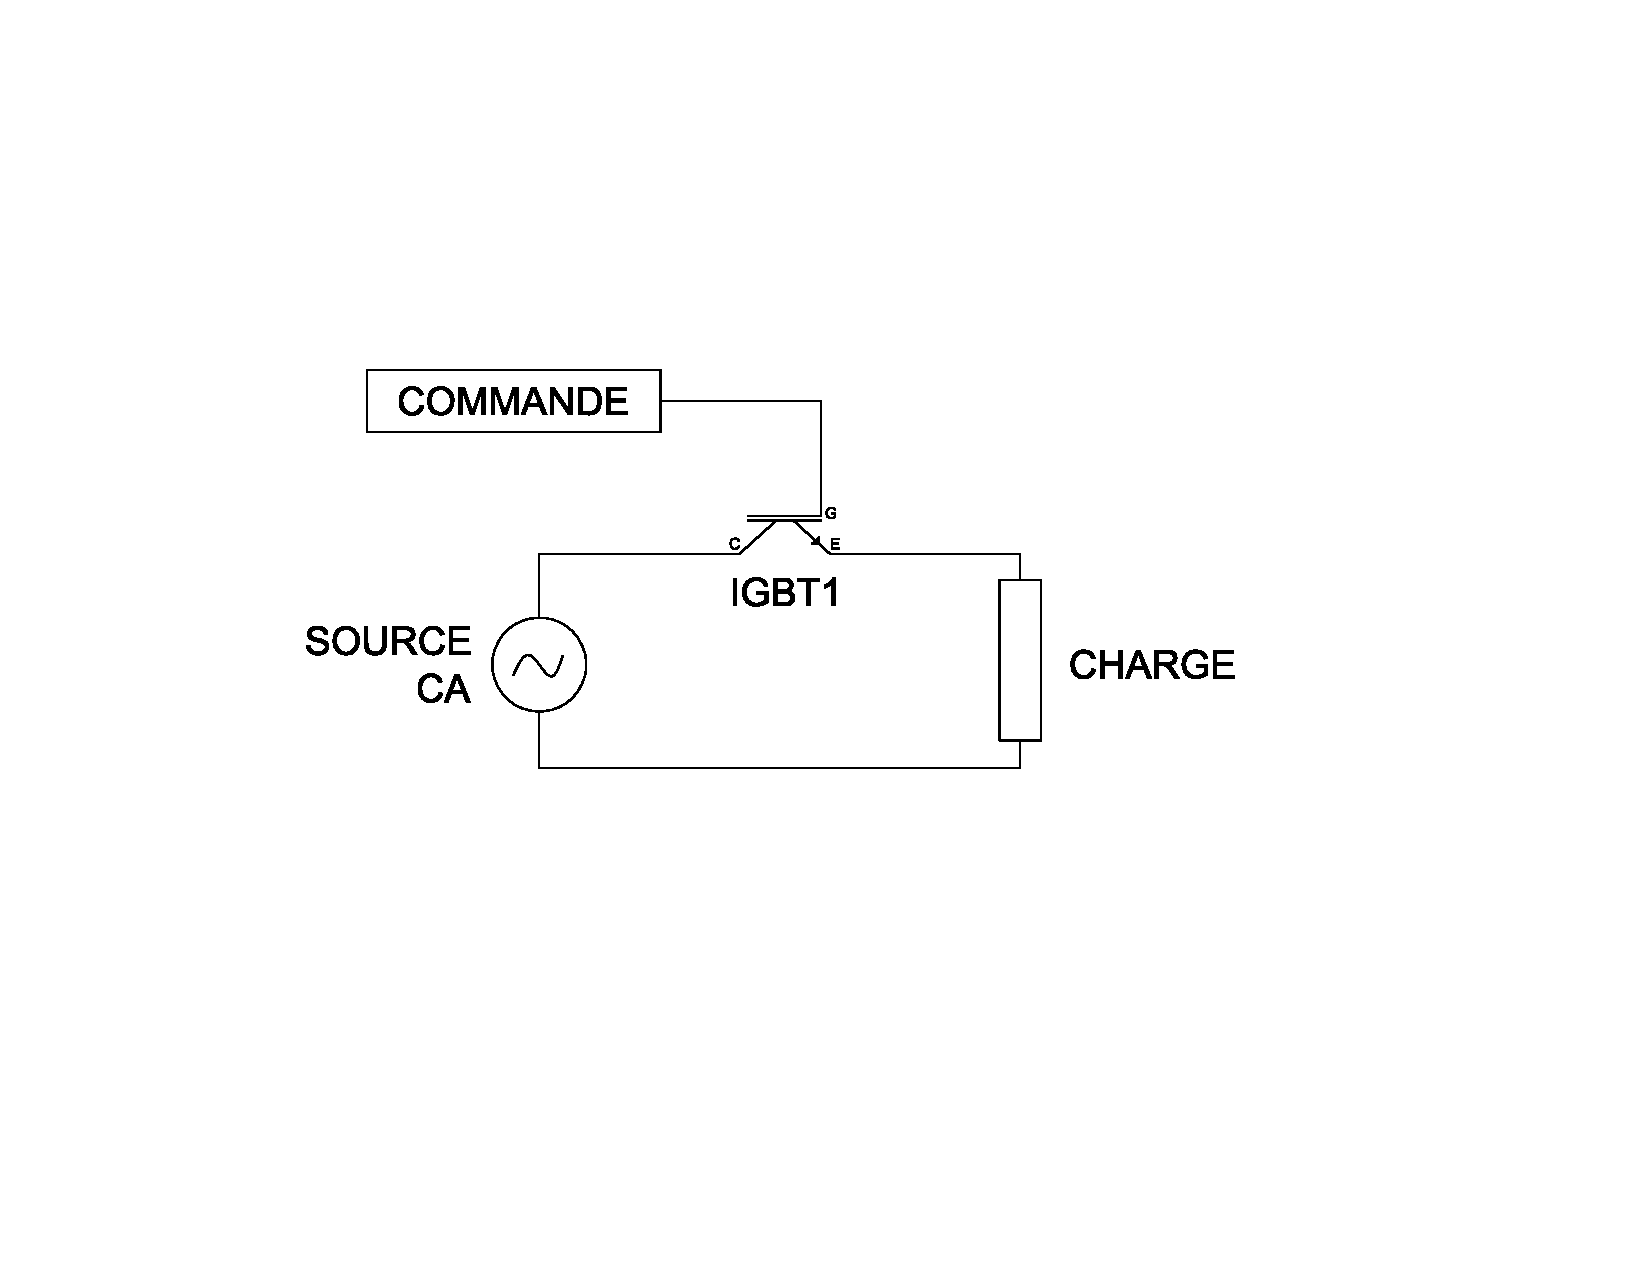
\includegraphics[width=0.7\textwidth]{Circuit/RedresseurMonophaseSimpleAlternanceIGBT}
		\caption{Circuit redresseur monophasé simple alternance avec IGBT et charge quelquonque}
		\label{fig:RedresseurMonophaseSimpleAlternanceIGBT}
	\end{center}   
\end{figure}


\begin{equation}
\label{eq:RLSimple}
v(t) = R i(t) + L \frac{d i(t)}{dt}
\end{equation}

Si l'on suppose la conduction continue de l'IGBT, il est possible d'exprimer le courant dans la charge en fonction de la tension de la source CA:

\begin{eqnarray}
V_{in}(t) &=& E_m\sin{\omega_0 t} \\
|Z| &=& \sqrt{R^2 + (\omega_0 L)^2} \\
\tau &=& \frac{L}{R}\\
\phi &=& \mbox{atan}(\omega_0 \tau) = \mbox{atan}(\omega_0 \frac{L}{R}) \\
\label{eq:solutionRLSimple} i(t) &=& \frac{E_m\sin{\phi}}{|Z|}\mbox{e}^{\frac{-t}{\tau}} + \frac{E_m\sin{(\omega_0 t + \phi})}{|Z|}\\
i(t=0) &=& i_0\\
i(t) &=& i_0  + \frac{E_m\sin{\phi}}{|Z|}\mbox{e}^{\frac{-t}{\tau}} + \frac{E_m\sin{(\omega_0 t + \phi})}{|Z|} \\
\end{eqnarray}

L'équation \ref{eq:solutionRLSimple} est la solution de l'équation différentielle \ref{eq:RLSimple} d'un circuit RL avec la partie de gauche qui est la solution transitoire (dépendante du circuit seulement) et la partie de droite qui est la solution en régime permanent (dépendante de l'excitation). 

\paragraph{}
La fonction principale de ce redresseur est de produire une tension et un courant qui sont strictement positifs. Dans le cas du redresseur simple alternance, seulement la partie positive de la source de courant alternative est envoyé à la charge et la partie négative est bloquée par l'IGBT qui agit comme une diode. De plus, du fait que l'IGBT est une source de courant commandée (sans pertes et sans délais pour les calculs théoriques) , il est possible de contrôler le temps de conduction de la partie positive du signal.

Ainsi, si l'on définit le temps total d'une période du signal par $T$, le temps de début de conduction de l'IGBT par $t_{on}$ et le temps de début de blocage par $t_{off}$, il est possible de définir le rapport de modulation $m = 2\cdot \frac{t_{off}-t_{on}}{T}$. Supposons un rapport de modulation $m_x$, il est possible, si l'on considère le courant initial nul et des temps de commutation nuls, d'exprimer le courant dans la charge RL pour une période $T$ donnée.

Les figures \ref{fig:RedresseurMonophaseSimpleAlternanceIGBTCourbes50} et \ref{fig:RedresseurMonophaseSimpleAlternanceIGBTCourbes100} présentent la tension et le courant dans la charge pour 2 différents niveaux de modulation. 

\begin{figure}
        \centering       
        \begin{subfigure}[Courant dans la charge en fonction de la tension dans la charge pour une modulation de 50\% avec un temps de début de conduction de 10\%]{
         		\label{fig:RedresseurMonophaseSimpleAlternanceIGBTCourbes50}
                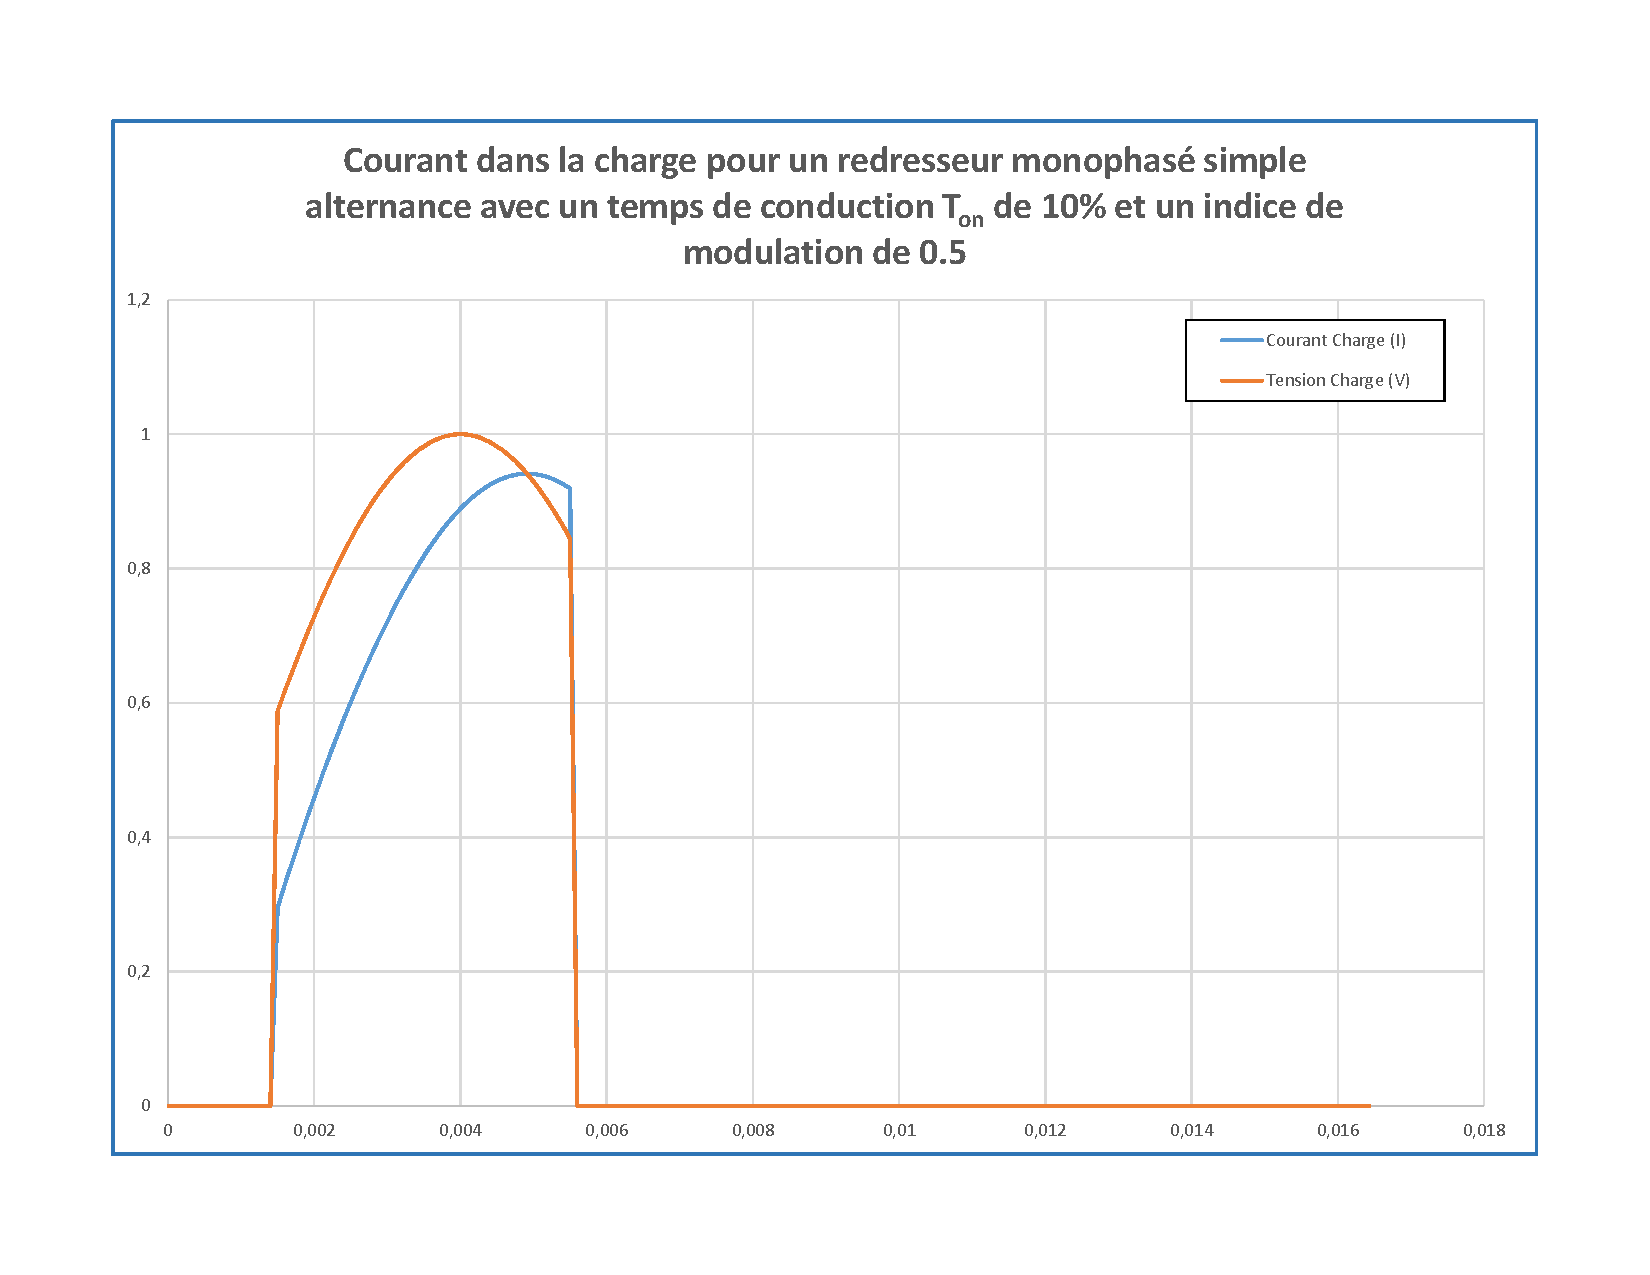
\includegraphics[width=0.68\textwidth]{Graphs/RedresseurMonophaseSimpleAlternance50}}
        \end{subfigure}        
        \begin{subfigure}[Courant dans la charge en fonction de la tension dans la charge pour une modulation de 100\% avec un temps de début de conduction de 0\%]{
         		\label{fig:RedresseurMonophaseSimpleAlternanceIGBTCourbes100}
                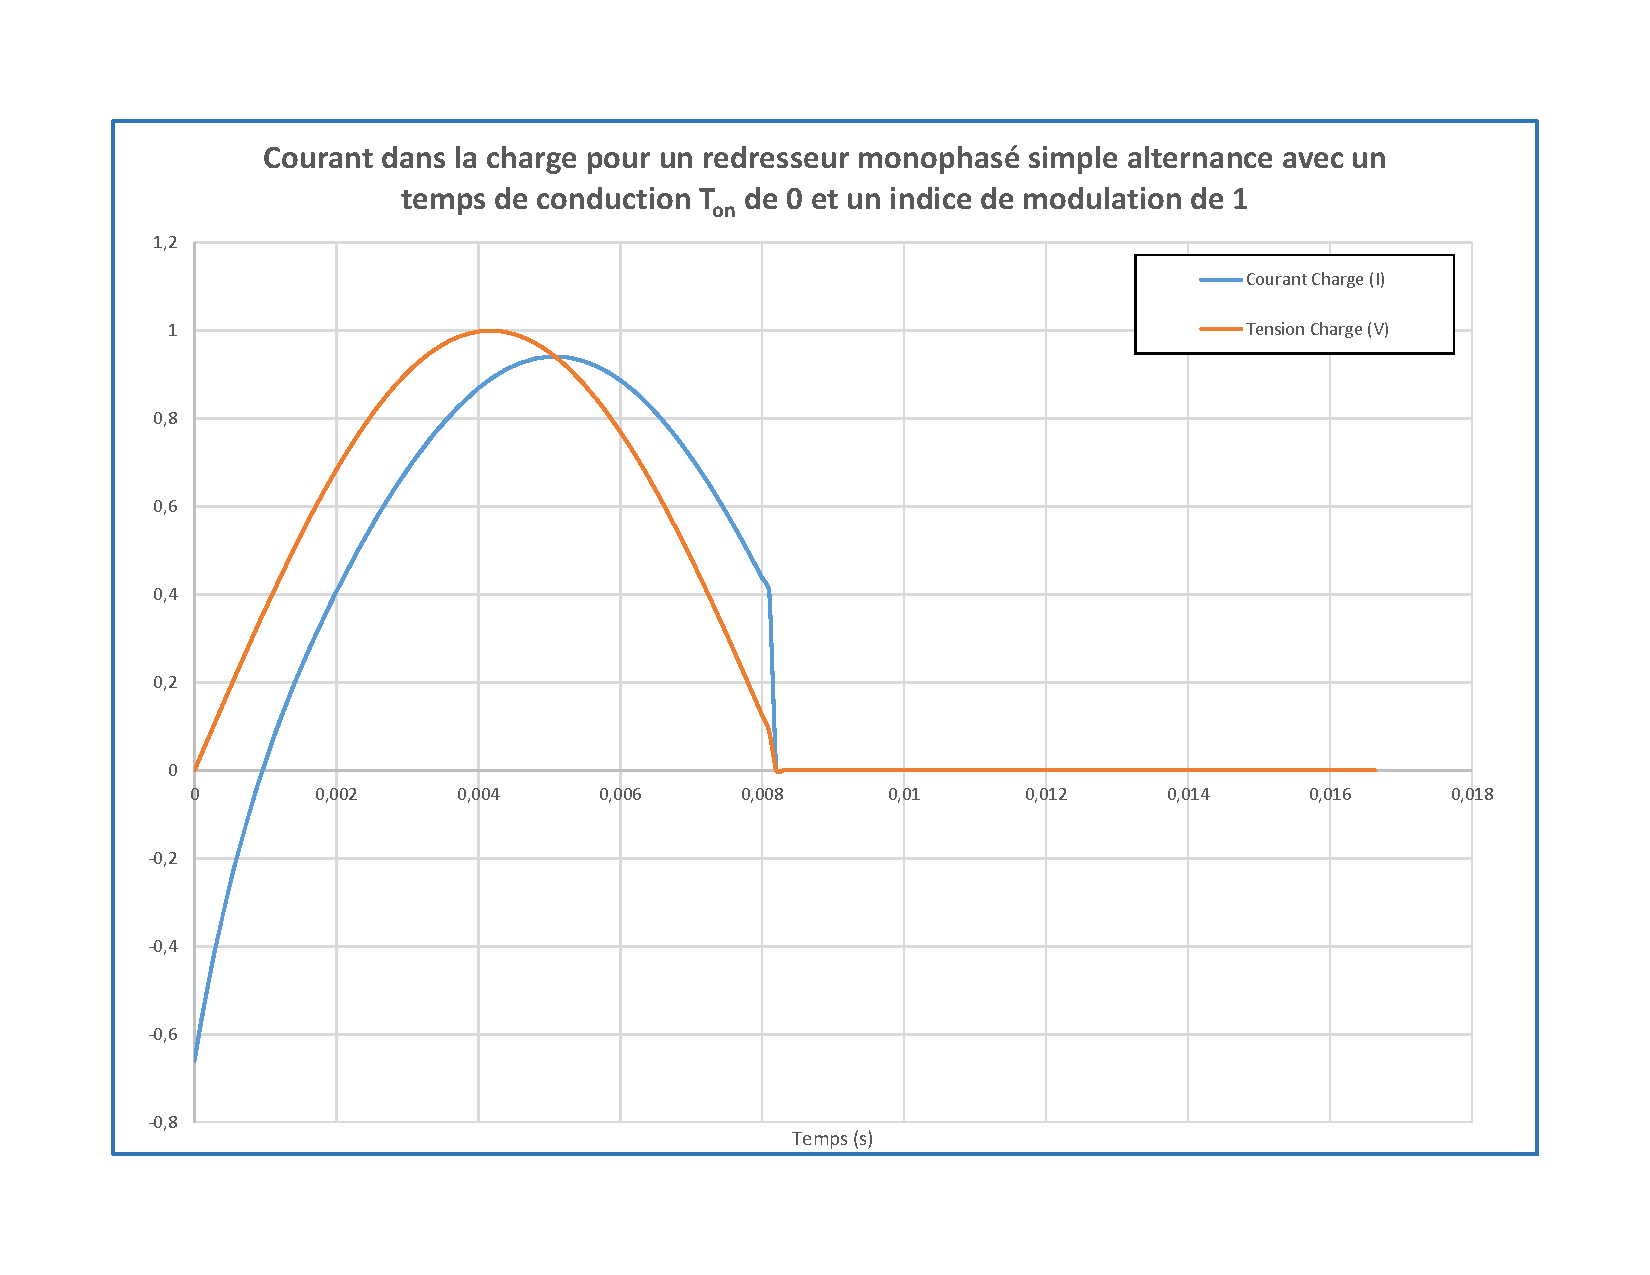
\includegraphics[width=0.68\textwidth]{Graphs/RedresseurMonophaseSimpleAlternance100}}
        \end{subfigure}
        \caption{Forme du courant et de la tension dans la charge pour 2 différents niveaux de modulation du redresseur monophasé à simple alternance}\label{fig:RedresseurMonophaseSimpleAlternanceIGBTCourbes}
\end{figure}

Comme la forme d'onde de tension et de courant dépendent entièrement du niveau de modulation choisi, il est intéressant d'obtenir les valeurs de tension et de courant moyen en fonction des paramètres de modulation. La valeur moyenne du courant sur une période se calcule comme suit :

\begin{eqnarray}
I_{moy} &=& \frac{1}{T}\int_{t_{on}}^{t_{off}} i(t) dt \\
I_{moy} &=& \frac{1}{T}\int_{t_{on}}^{t_{off}} \left( \frac{E_m\sin{\phi}}{|Z|}\mbox{e}^{\frac{-t}{\tau}} + \frac{E_m\sin{(\omega_0 t + \phi})}{|Z|}\right) dt \\
I_{moy} &=& \frac{E_m}{T} \left( \frac{-\mbox{e}^{-\frac{t_{off}}{\tau}}\sin{(\phi)}\omega_0 \tau + \mbox{e}^{-\frac{t_{on}}{\tau}} + \cos{(\omega_0 t_{on} + \phi)}-\cos{(\omega_0 t_{off} + \phi)}}{|Z|\omega_0} \right)
\end{eqnarray}

Par la suite, la valeur moyenne de la tension se calcule comme suit : 
\begin{eqnarray}
V_{moy} &=& \frac{1}{T}\int_{t_{on}}^{t_{off}} V_{in}(t) dt \\
V_{moy} &=& \frac{1}{T}\int_{t_{on}}^{t_{off}} (E_m \sin{\omega_0 t}) dt \\
V_{moy} &=& \frac{E_m}{T} \left( \frac{\cos{(\omega_0 t_{on})} - \cos{(\omega_0 t_{off})}}{\omega_0} \right)
\end{eqnarray}

\section{Fonctionnement d'un redresseur monophasé double alternance}
Cette section a pour objectif de décortiquer le fonctionnement d'un redresseur monophasé à double alternance réversible en courant et en tension, composé d'une source de courant sinusoïdale parfaite, de 4 interrupteurs de type IGBT (avec diodes en antiparallèle) et d'une charge quelconque. Le montage analysé est présenté à la figure à la figure \ref{fig:RedresseurMonophaseDoubleAlternanceIGBT}. Le principal avantage de ce type de redresseur par rapport au redresseur simple alternance est la possibilité d'inverser la partie négative du signal alternatif et de permettre la réversibilité en courant et en tension. En effet, lors de la partie positive de l'onde, les IGBT 1 et 3 vont s'activer ce qui va permettre d'alimenter la charge avec une tension positive et lors de la partie négative de l'onde, les IGBT 2 et 4 vont conduire et ainsi alimenter la charge avec une tension redressée. 

\begin{figure}[htb!]
  \begin{center}  
    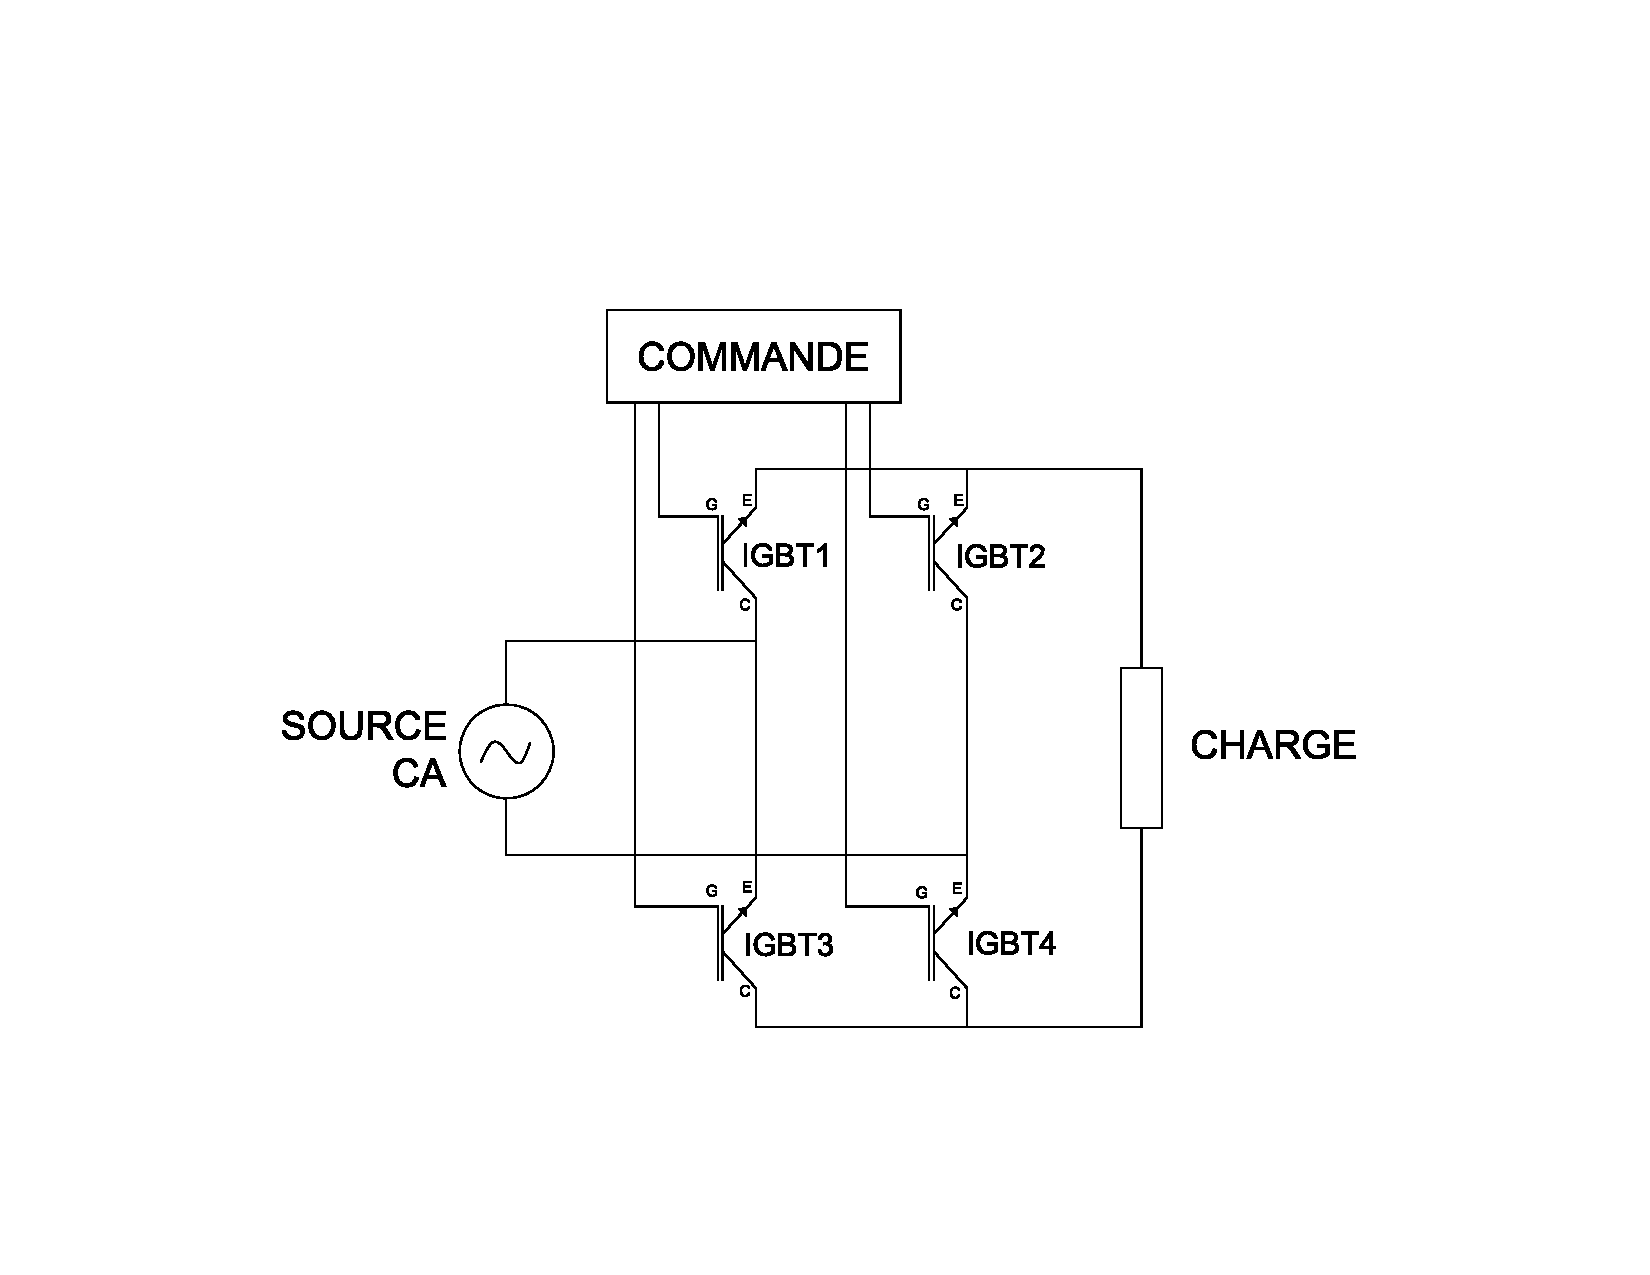
\includegraphics[width=0.7\textwidth]{Circuit/RedresseurMonophaseDoubleAlternanceIGBT}
    \caption{Circuit redresseur monophasé double alternance avec IGBT et charge quelquonque}
    \label{fig:RedresseurMonophaseDoubleAlternanceIGBT}
  \end{center}   
\end{figure}

\paragraph{}
La présence de l'alternance négative redressée permet deux modes de conduction, soit le mode continu et le mode discontinu. Comme les équations du système en régime permanent sont différentes dans les deux modes, il est nécessaire d'effectuer la résolution pour les deux différents cas.

\subsection{Mode continu}
Le redresseur double alternange opère dans le mode continu lorsque le courant dans la charge ne retombe jamais à zero. Ainsi, il est nécessaire d'adapter l'équation \ref{eq:solutionRLSimple} trouvée dans la section précédente. Nous savons que le courant dans la charge RL, une fois l'inductance chargée, est donné par :

\begin{eqnarray}
\label{eq:RedresseurMonophaseDoubleAlternanceContinu1}
i(t) &=& C_1\mbox{e}^{\frac{-t}{\tau}} + \frac{E_m\sin{(\omega_0 t - \phi})}{|Z|}
\end{eqnarray}

Où:
\begin{eqnarray}
C_1 &=& \left( I_1 - \frac{E_m\sin{(\omega_0 t + \phi})}{|Z|}\right)\mbox{e}^{\left(\frac{R}{L}\right)\left(\frac{\pi}{\omega_0}\right)}
\end{eqnarray}

En appliquant la condition $I_L(\omega_0 t = 0)=I_L(\omega_0 t=\pi)=I_1$ dans l'équation \ref{eq:RedresseurMonophaseDoubleAlternanceContinu1}, nous trouvons que :
\begin{equation}
\label{eq:RedresseurMonophaseDoubleAlternanceContinu2}
	I_1 = \frac{E_m\sin{(\phi)}}{|Z|}  \frac{1 + \mbox{e}^{\frac{-1}{\tau}}}{1 - \mbox{e}^{\frac{-1}{\tau}}}
\end{equation}

Finalement en remplaçant $I_1$ dans l'équation \ref{eq:RedresseurMonophaseDoubleAlternanceContinu1} par l'équation \ref{eq:RedresseurMonophaseDoubleAlternanceContinu2}, nous trouvons que le courant dans la charge pour chaque demi-période, une fois l'inductance chargée, est donné par :

\begin{equation}
	i(t) = \frac{E_m}{|Z|}\left[\sin{(\omega_0 t - \phi)} + \frac{2\sin(\phi) \mbox{e}^{\frac{-t}{\tau}}}{1-\mbox{e}^{\left(\frac{R}{L}\right)\left(\frac{\pi}{\omega_0}\right)}} \right] 
\end{equation}

\subsection{Mode discontinu}
Le redresseur double alternange opère dans le mode discontinu lorsque le courant dans la charge peut retomber à zero. Ainsi, il est nécessaire d'adapter l'équation \ref{eq:solutionRLSimple} trouvée dans la section précédente. Nous savons que le courant dans la charge RL ,une fois l'inductance chargée, est donné par :

\begin{eqnarray}
\label{eq:RedresseurMonophaseDoubleAlternanceContinu1}
i(t) &=& C_1\mbox{e}^{\frac{-t}{\tau}} + \frac{E_m\sin{(\omega_0 t - \phi})}{|Z|}
\end{eqnarray}

Où:
\begin{eqnarray}
C_1 &=& \left( I_1 - \frac{E_m\sin{(\omega_0 t + \phi})}{|Z|}\right)\mbox{e}^{\left(\frac{R}{L}\right)\left(\frac{\pi}{\omega_0}\right)}
\end{eqnarray}

En appliquant la condition $I_L(\omega_0 t = 0)=I_L(\omega_0 t=\pi)=I_1$ dans l'équation \ref{eq:RedresseurMonophaseDoubleAlternanceContinu1}, nous trouvons que :
\begin{equation}
\label{eq:RedresseurMonophaseDoubleAlternanceContinu2}
	I_1 = \frac{E_m\sin{(\phi)}}{|Z|}  \frac{1 + \mbox{e}^{\frac{-1}{\tau}}}{1 - \mbox{e}^{\frac{-1}{\tau}}}
\end{equation}

Finalement en remplaçant $I_1$ dans l'équation \ref{eq:RedresseurMonophaseDoubleAlternanceContinu1} par l'équation \ref{eq:RedresseurMonophaseDoubleAlternanceContinu2}, nous trouvons que le courant dans la charge pour chaque demi-période, une fois l'inductance chargée, est donné par :

\begin{equation}
	i(t) = \frac{E_m}{|Z|}\left[\sin{(\omega_0 t - \phi)} + \frac{2\sin(\phi) \mbox{e}^{\frac{-t}{\tau}}}{1-\mbox{e}^{\left(\frac{R}{L}\right)\left(\frac{\pi}{\omega_0}\right)}} \right] 
\end{equation}

\section{Fonctionnement d'un redresseur triphasé double alternance}
Cette section a pour objectif de décortiquer le fonctionnement d'un redresseur triphasé à double alternance réversible en courant et en tension, composé de 3 sources de courant sinusoïdale parfaites, de 6 interrupteurs de type IGBT(avec diodes en antiparallèle) et d'une charge quelconque. Le montage analysé est présenté à la figure à la figure INSÉRER FIGURE REDRESSEUR 3$\Phi$ ici. Ce montage est analogue à celui présenté à la section précédente et permet de diminuer l'ondulation vue à la charge. Il est réversible en courant et en tension, tout comme le montage précédent. Seule l'utilisation en régime permanent (régulation de tension) sera présentée dans ce document, le développement mathématique utile pour la compréhension fondamentale ayant été présenté plus tôt. Dans cet exemple, on suppose une charge $RC$, dont la résistance correspond à la valeur nominale de la puissance moyenne débitée par le redresseur. Si l'on suppose un condensateur C, initialement chargé à une tension désirée, une source de courant parfaite côté réseau, des commutations instantanées et sans pertes et que l'on néglige les snubbers, il est possible de dresser un portrait mathématique simple du redresseur. La fonction de transfert d'un circuit $RC$ dans le domaine de Laplace est donnée par l'équation suivant:
\begin{equation}
H(s) = \frac{R}{RCs + 1}
\end{equation}
Il est possible de supposer que le courant injecté par chaque bras du redresseur dans la charge est modulable selon le temps de conduction de l'IGBT concerné selon la phase du signal par rapport aux autres (seul le montage dont la tension est supérieure (en valeur absolue) aux autres s'amorce. La période de conduction totale et maximale d'un IGBT est de 60 degrés, sur une période totale de 360 degrés. Pour simplifier l'analyse, on peut analyser le montage comme 6 montages redresseurs monophasés simple alternance et ne se concentrer que sur un IGBT. Par ailleurs, on peut négliger l'ondulation liée à la nature sinusoïdale de la charge et approximer par la valeur moyenne d'un sinus sur cette période, que l'on calcule comme suit (fonctionnement pleine onde):
\begin{equation}
I_{moy} = \frac{3}{\pi}\int_{60}^{120} I_M \sin(\theta)d\theta = \frac{3I_M}{\pi}\left( \cos(60)-\cos(120)\right) = \frac{3I_M}{pi}
\end{equation}
On trouve par la suite que selon l'indice de modulation ($m_x$) sur la période de 60 degrés donnée et ce, pour une fréquence de modulation de $f_{mod} = \frac{1}{T_{mod}}$ on peut approximer le courant dans la charge par $I_{CH} = \frac{3I_M m_x}{pi}$. Pour le reste de la période de modulation, on a 0A. Pour une période de modulation, la tension vue à la charge est donnée par l'équation suivante dans le domaine de Laplace:
\begin{equation}
V(s) = \frac{R\cdot I_{CH}}{RCs + 1} \left(\frac{1 - e^{-m_xT_{mod}s}}{s}\right) = R\cdot I_{CH}\frac{1/RC}{s(s + 1/RC)} - R\cdot I_{CH}\frac{1/RC}{s(s + 1/RC)}e^{-m_xT_{mod}s}
\end{equation}
On peut par la suite effectuer la transformation dans le domaine du temps en supposant qu'on applique un courant à un moment quelconque
\begin{equation}
v(t) = R\cdot I_{CH}\left((1-e^{-(t-t_0)/RC})u(t-t_0) - (1-e^{t-(m_xT_{mod}-t_0)/RC})u(t-m_xT_{mod}-t_0)\right) + v_C(t_0)
\end{equation}
Pour une période de conduction de 60$^\circ$, donc de 3.33ms à 50Hz et un temps de modulation de 1ms, il est possible de calculer le courant dans un interrupteur. On sait premièrement que la puissance nominale du montage étudié est de 2.7MW à 5000V. On calcule donc une résistance équivalente R étant égale à 9.26$\Omega$ et un courant DC moyen de 540A à la charge. Le banc de condensateurs est fixe à 330mF. On suppose que l'origine du temps est à 0s. Connaissant la forme de la tension à la charge, il est possible de déterminer le courant traversant la résistance en fonction du temps si l'on considère une source de courant idéale à l'entrée:
\begin{equation}
i_R(t) = I_{CH}(1-e^{-(t)/RC})u(t) - I_{CH}(1-e^{t-(m_xT_{mod})/RC})u(t-m_xT_{mod}) + v_C(0)/R
\end{equation}
On considère maintenant le système en régime permanent et on cherche  à ce que l'indice de modulation soit tel que la moyenne du courant soit le courant nominal. Le courant de source crête est égal à $I_M = \sqrt(2/3)V_{AC} = 2000\sqrt{2/3} = 1633A$ et donc le courant moyen de charge égal à $I_{CH} = \frac{3I_M m_x}{pi} = \frac{2000\sqrt(6)m_x}{\pi} = 1559.39m_xA$. On désire un courant moyen dans la charge de 540A. , il est alors nécessaire que l'indice de modulation soit de 0.346. 
Par ailleurs, le redresseur est en mesure de fournir jusqu'à 3.6MW de puissance crête et ce, au moment où la tension du bus CC chute à environ 3.2kV. On peut donc calculer l'indice de modulation à cette puissance de la même manière que précédemment et on obtient 0.721, soit un courant moyen de 1125A à la charge. Il est à noter qu'en pratique on régule l'amplitude du courant côté réseau en imposant une référence de courant d'amplitude variable qui permet d'imposer l'indice de modulation approprié.

Dans le cas où la puissance demandée est maximale, il est possible de calculer une approximation des valeurs de courants RMS vues par les interrupteurs et de les comparer à celles prévues par le manufacturier. On a premièrement que le courant maximal (en valeur moyenne) débité par la source idéale (côté réseau) est de 1559.39A. Il est possible de calculer la valeur RMS maximale sur la période de conduction d'un IGBT en connaissant l'indice de modulation. Soit $m_x = 0.721$, on a que:

\begin{equation}
I_{RMS} = \sqrt{\int_0^{m_x} I_{CH}^2} = \sqrt{m_x}I_{CH}  \sqrt{0.721}I_{CH}= 1324A
\end{equation}

Sur l'ensemble d'une période du signal, on a donc:
\begin{equation}
I_{RMS} =  \sqrt{1/6\int_0^{m_x} I_{CH}^2} = \frac{1}{\sqrt{6}}\cdot 1324A = 540.52A
\end{equation}

En fonctionnement à puissance nominale, on trouve que le courant RMS pendant la conduction est donné par:
\begin{equation}
I_{RMS} =  \sqrt{m_x}I_{CH} = \sqrt{0.346}I_{CH} = 917.26A
\end{equation}

Sur l'ensemble d'une période du signal, on a donc:
\begin{equation}
I_{RMS} =  \sqrt{1/6\int_0^{m_x} I_{CH}^2} = \frac{1}{\sqrt{6}}\cdot 917.26A = 374.47A.
\end{equation}
\section{Fonctionnement d'un redresseur triphasé 3 niveaux NPC}
Le projet implanté au CERN emploie un redresseur triphasé à 3 niveaux NPC dont le schéma est présenté à la figure INCORPORER FIGURE AFE 3L ici. L'avantage de cette configuration par rapport à la précédente est au niveau de la tension vue aux bornes des interrupteurs. En fonctionnement normal, l'ajout d'un niveau supplémentaire divise par 2 la tension commutée par les interrupteurs, ce qui permet d'avoir des composantes de dimensions inférieures. Au point de vue logique et commande, les calculs théoriques approximatifs tiennent toujours, le fonctionnement  de base est pratiquement inchangé du point de vue du courant. Cependant, dans cette configuration, les interrupteurs conduisent par paires dans chaque bras, ce qui modifie la commande à appliquer. De plus, l'ajout d'un point milieu \og clampé \fg{} par des diodes modifie substantiellement la stabilité de la tension 0 dans cette configuration. les séquences d'enclenchement des niveaux vont perturber la tension de neutre. En pratique, cette tension doit être équilibrée par un circuit de commande auxiliaire. Aussi, il faut donc dimensionner les interrupteurs de manière à pouvoir commuter la moitiée de la tension du bus CC de  5kV, soit 2.5kV. Le bus CC pouvant monter jusqu'à 5.1kV, il est nécessaire de dimensionner les IGBT pour obtenir une tension de 2.75kV en répétition à leurs bornes.